%%%%%%%%%%%%
%
% $Autor: Wings $
% $Datum: 2019-03-05 08:03:15Z $
% $Pfad: NAgicWand,tex $
% $Version: 4250 $
% !TeX spellcheck = en_GB/de_DE
% !TeX encoding = utf8
% !TeX root = filename 
% !TeX TXS-program:bibliography = txs:///biber
%
%%%%%%%%%%%%


\chapter{Magic Wand}



\begin{itemize}
  \item Als Mikrocontrollerboard wird ein Arduino Nano 33 BLE verwendet:
    
          \URL{https://docs.arduino.cc/hardware/nano-33-ble/}
  \item Betrieben wird das Controllerboard mit einer Lithium Batterie CR2032: \cite{Energizer:2018}
  
        \URL{https://data.energizer.com/pdfs/cr2032.pdf}           
        
  \item Der Stab ist aus Acryl: 
  
        \URL{https://acrylhaus.com/Rundstab-aus-Acrylglas-XT-mit-Luftblasen}
  \item Für den 3D-Druck wurde PETG Filament verwendet:
  
      \URL{https://www.material4print.de/filament/petg/31/petg-tiefschwarz?c=15}
            
\end{itemize}


\section{Attention}

An drei Ausgangpins des Controllerboards ist, über Vorwiderstände von 180 Ohm, eine RGB-LED
angeschlossen.

Der Zauberstab lässt sich über die eingebaute Micro-USB Schnittstelle programmieren.

Dazu muss der Zauberstab geöffnet und der Jumper im inneren geschlossen (gesteckt werden).


\textbf{ACHTUNG vor dem Stecken des Jumpers muss der Stab ausgeschaltet sein und er darf
nicht eingeschaltet werden, solange der Jumper steckt!!}


\section{Gehäuse}


\includegraphics[width=0.8\textwidth]{MagicWand/MagicWandS}

\bigskip

Die Gehäusekonstruktion wurde mit Fusion 360 erstellt.

\bigskip

\includegraphics[width=0.3\textwidth]{MagicWand/MagicWandCAD01}
\includegraphics[width=0.3\textwidth]{MagicWand/MagicWandCAD02}
\includegraphics[width=0.3\textwidth]{MagicWand/MagicWandCAD03}

\bigskip

{
  \captionof{code}{Einschalten der Farben der RGB-Led}
  \ArduinoExternalO{../../Code/Nano33BLESense/MagicWand/MagicWandOnOff.ino}
}


{
  \captionof{code}{Farbwechsel der RGB-Led}
  \ArduinoExternalO{../../Code/Nano33BLESense/MagicWand/MagicWandPWM.ino}
}


\chapter{Magic Wand project}

Magic Wand project, our aim is to create a magic wand capable of recognizing 4 different movements and changing color with each one. 

The magic wand project developed by google and using the TensorFlow tool can recognize different movements. Our project is based on the project developed by Google, then modified to suit us. 

TensorFlow is an AI application, this AI tools can used in lot of project, with Arduino IDE, the library \PYTHON{Arduino\_TensorFlowLite} is composed with 5 examples of application, during this project we focus on one specific application, the Magic Wand.

The TensorFlow tool is used for recognition of motion and the TensorFlow Lite is used for this library. 

During my reflexion about the project I used the book named TinyML: Machine Learning with TensorFlow Lite on Arduino and Ultra-Low-Power Microcontrollers \cite{Warden:2020} and the book IoT Projecty with Arduino Nano 33 BLE Sense. \cite{Kurniawan:2021b}.

\section{Library download}

The library \FILE{TensorFlow Lite} is an compagnie library, to have this library you need to download a zip file "tensorflow\_lite\_20\_02\_25", \cite{GoogleTensorFlow:2019}, the last update was doing on February 2020.  The figure \ref{Figure:TensorFlowLite} was a print of Google Codelabs site who treat about the libraryTensorFlow Lite.

\begin{center}
    \includegraphics[width=10cm]{MagicWand/flowlite.png}
    \captionof{figure}{TensorFlow Lite}\label{Figure:TensorFlowLite}
\end{center}

After download the library of TensorFlow Lite on zip file, we need to used this file and put on Arduino IDE library. The figure \ref{Figure:TensorFlowLiteLib} show how library was been adding with : \menu{Sketch>Include library>Add .zip library}


\begin{center}
    \includegraphics[width=10cm]{MagicWand/ziplib.png}
    \captionof{figure}{Adding the library  TensorFlow Lite}. \label{Figure:TensorFlowLiteLib}	
\end{center}


\section{Introduction}

The project we're studying is a magic wand developed by Google, and we need to understand it in order to adapt it to our needs. Once we've understood the project, we'll also be able to study the library \FILE{TensorFlow Lite}. This chapter will explain how the Magic Wand project works in several points, explaining each part of the program. Once we've understood the program, we'll go on to explain how it works and what modifications need to be made to adapt it to the nano 33 BLE Sense.

\bigskip 

The project can be found using the library \FILE{TensorFlow Lite} example. 

The project is composed by 13 majors files in addition to files TensorFlow: 

\begin{itemize}
    \item \FILE{constants.h}
    \item \FILE{accelerometer\_handler.h}
    \item \FILE{arduino\_accelerometer\_handler.cpp}
    \item \FILE{output\_handler.h}
    \item \FILE{arduino\_output\_handler.cpp}
    \item \FILE{gesture\_predictor.h}
    \item \FILE{gesture\_predictor.cpp}
    \item \FILE{arduino\_main.cpp}
    \item \FILE{magic\_wand.ino}
    \item \FILE{magic\_wand\_ model\_data.cpp}
    \item \FILE{magic\_ wand\_model\_data h}
    \item \FILE{main\_functions.h}
    \item \FILE{version.h}
    
\end{itemize}

This chapter will help us to understand the different parts of these files, the 13 files will be developed in order to understand each part of the code. You'll then be able to take a more global view of the project. To find out how to modify the google magic wand project for our project. 

\begin{center}
    \includegraphics[width=10cm]{MagicWand/MagicWand.png}
    \captionof{figure}{Magic Wand example}
\end{center}



\section{Magic Wand explanation}
The project is made up of several sub-projects. The main part compiles and assembles data. The project is made up of a number of sub-projects, each of which has a purpose that will be described throughout the project. 

\begin{center}
    \captionof{code}{Magic Wand main explain }
    \ArduinoExternal{firstline=15,lastline=31}{../../Code/Nano33BLESense/magic_wand_code/magic_wand.ino}
    \label{Magic Wand Flow Lite General}
\end{center}


\subsection{File \PYTHON{constant.h}}

This part explain basic number of gesture, how many gesture we have. This example explain the time and the number  of prediction he had on his memory.  

\bigskip

We have 4 basics gestures with numeration : 

\begin{itemize}
    \item Wing = 0  
    \item Ring = 1
    \item Slope = 2
    \item Unknwon - None = 3	
\end{itemize} 

\begin{center}
    \captionof{code}{Constant of magic wand}
    \ArduinoExternal{firstline=16,lastline=27}{../../Code/Nano33BLESense/magic_wand_code/constants.h}
    \label{MagicWandConstant}
\end{center}

The detection Threshold is 0.6 (f in the code is for float). The memory prediction lenght is 5 and the predection was delete avec 25 seconde. 

\begin{center}
    \captionof{code}{Constant of magic wand}
    \ArduinoExternal{firstline=34,lastline=38}{../../Code/Nano33BLESense/magic_wand_code/constants.h}
    \label{Magic Wand Constant}
\end{center}


\subsection{File \PYTHON{Accelerometer\_handler.h}}

This part of the project is used to manage the accelerometer. If this part is not correctly defined, it needs to be for the project to run smoothly. 

\begin{center}
    \captionof{code}{Magic Wand accelerometer handler explain}	
    \label{Figure:MagicWandAccelerometerhandler}
    \ArduinoExternal{firstline=16,lastline = 30} {../../Code/Nano33BLESense/magic_wand_code/accelerometer_handler.h}	
\end{center}


\PYTHON{\#ifndef} is a function which works like an if and endif except that here it looks to see if a function is defined. If it is, the program skips, otherwise it continues on the next lines.In this code they check if 
\PYTHON{TENSORFLOW\_LITE\_MICRO\_EXAMPLES\_MAGIC\_WAND\_ACCELEROMETER} is define. If it's wasn't define they define this function and define 2 libraries :  \FILE{tensorflow/lite/c/common.h} and  \FILE{tensorflow/lite/micro/micro\_error\_reporter.h}. 

They also define begin\_index and change the status in error\_reporter until. The \PYTHON{\#ifndef} finished when we arrived at the \PYTHON{\#endif}.


\subsection{\PYTHON{Arduino\_accelerometer\_handler.h}}

\begin{center}
    \captionof{code}{Magic Wand Arduino Accelerometer explain}
    \ArduinoExternal{firstline=16,lastline= 32}{../../Code/Nano33BLESense/magic_wand_code/arduino_accelerometer_handler.cpp}
    \label{MagicWandArduinoAccelerometerHandler}		
\end{center}

In the first part we include the file and library, we had : 
\begin{itemize}
    \item \FILE{accelerometer\_hander.h}: It was been define above
    \item \FILE{Arduino.h}: It's the hardware part for used on arduino 
    \item \FILE{Arduino\_LSM9DS1.h}: It's the part for library accelerometer 
    \item \FILE{constant.h}: It's constant who was used to define gesture number.  
\end{itemize}

In this part they reset data with \PYTHON{sava\_data[600] = {0.0}}, made a begin position \PYTHON{begin\_index= 0}, they also do variable if the system wasn't run and how many measurements they saved in this memory. 

The \PYTHON{pending\_initial\_data} = true check for the data if they have enought or not data.  \PYTHON{The sample\_every\_n} is a number of measurement during the downsampling. 

\begin{center}
    \captionof{code}{Magic Wand Arduino Starting Accelerometer}		
    \ArduinoExternal{firstline=34,lastline= 54}{../../Code/Nano33BLESense/magic_wand_code/arduino_accelerometer_handler.cpp}
    \label{Magic Wand Arduino Starting Accelerometer}
\end{center}


The \PYTHON{SetupAccelerometer} have pointer type ErrorReporter on error\_reporter if they doesn't work. When the IMU is not initilized, we have an error \textcolor{violet}{Failled to initialize IMU} and they return value \PYTHON{kTfLiteError}. 
After the IMU change this mode, he going in continuous mode, that a type of always on mode.  

The constant \PYTHON{sample\_rate} take information of \PYTHON{IMU.accelerationSampleRate}  and with \PYTHON{sample\_every\_n} this function calculates sampling frequency with Euclidean division.

Now they can start and \textcolor{violet}{Magic Start}, \PYTHON{kTfLiteOk} was return. 

\begin{center}
    \captionof{code}{Magic Wand Arduino Read Accelerometer }		\ArduinoExternal{firstline=56,lastline= 72}{../../Code/Nano33BLESense/magic_wand_code/arduino_accelerometer_handler.cpp}
    \label{Code: Magic Wand Arduino Read Accelerometer}
\end{center}


The first ligne the function \PYTHON{ReadAccelerometer} define error in his answer. They blocks new data appearing.  The \PYTHON{IMU.readAccelerometer(x,y,z)} data is check. If we had \PYTHON{IMU.readAcceleration(x,y,z)} is different with 0,we can read the data, if the \PYTHON{IMU.readAcceleration(x,y,z)} is 0, we had error message \textcolor{violet}{Failed to read data}. 

The \PYTHON{sample\_skip\_counter} change to had the same value with \PYTHON{sample\_every\_n}. 

\begin{center}
    \captionof{code}{Magic Wand Arduino Accelerometer handler read data}		\ArduinoExternal{firstline=93,lastline= 111 }{../../Code/Nano33BLESense/magic_wand_code/arduino_accelerometer_handler.cpp}
    \label{Magic Wand Arduino Accelerometer handler read data}
\end{center}

This first line is to change the coordonate because with this position we have a difference with tool referencial and your referencial. The values are multiplied by 100 because they are micro movements.The cumptor lign we had a reset index ligne if index is full and they create new\_data. 

\begin{center}
    \captionof{code}{Magic Wand Arduino Accelerometer handler read data}		\ArduinoExternal{firstline=113,lastline= 133} {../../Code/Nano33BLESense/magic_wand_code/arduino_accelerometer_handler.cpp}
    \label{Magic Wand Arduino Accelerometer handler read data}
\end{center}

The \PYTHON{pending\_inital\_data} is used to waiting about the initialized data.
We check with \PYTHON{pending\_inital\_data \& \& begin\_index} '>=' 200 they check if they had all data. 
The function \PYTHON{for(int i= 0; i < lenght; i++){};} was used to \PYTHON{sava\_data} in the good sense because when \PYTHON{IMU.ReadAccelerometer()} read the first value is at the end and the old value is the first, with this function they invesed this and frist value is on the first, the second on the second,... this was save on \PYTHON{input[i]}.

\subsection{File \PYTHON{Output\_handler.h}}

The function \PYTHON{\# ifndef} TENSORFLOW\_LITE\_MICRO\_EXAMPLES\_MAGIC\_WAND\_OUTPUT\_HANDLER\_H\_ is checked, we see if it's defined, if not we define it and then we include the functions common.h and micro\_error\_reporter.h, the HandleOutput function is also defined at the same time. 

\begin{center}
    \captionof{code}{Magic Wand Arduino  output handler }		\ArduinoExternal{firstline=16,lastline= 24 }{../../Code/Nano33BLESense/magic_wand_code/output_handler.h}
    \label{Magic Wand Arduino  output handler}
\end{center}

\subsection{File \PYTHON{arduino\_output\_handler.cpp}}

The test checks whether the \PYTHON{is\_initalized} function is set to 0 or 1. If it is set to 1, the program is initialized if it is set to 0, the program initializes, outputs the \PYTHON{LED\_BUILTIN} and declares \PYTHON{is\_initialized}. Note that if \PYTHON{is\_initilized} is set to 0, then the if loop is launched as the inverse of \PYTHON{is\_initialized}.  

The second part of the program is designed to recognize the 3 types of gestures in addition to none: W, O and SLOPE. They are described as a point cloud that can be compared with data obtained from future movements or printed on an serial monitor. 


\begin{center}
    \captionof{code}{Magic Wand Arduino output handler}		\ArduinoExternal{firstline=16,lastline= 56 }{../../Code/Nano33BLESense/magic_wand_code/arduino_output_handler.cpp}
    \label{Magic Wand Arduino output handler}
\end{center}



\subsection{File \PYTHON{gesture\_predictor.h}}


The function \PYTHON{\# ifndef} check if  TENSORFLOW\_LITE\_MICRO\_EXAMPLES\_MAGIC\_WAND\_GESTURE\_PREDICTOR\_H\_ is define, if it's defined they go to \PYTHON{\#endif}, if not we define it and they include new functions \PYTHON{PredictGesture}, this function have for parameter (conts float * prediction\_socres).

\begin{center}
    \captionof{code}{Magic Wand gesture predictor}		\ArduinoExternal{firstline=16,lastline= 49 }{../../Code/Nano33BLESense/magic_wand_code/gesture_predictor.h}
    \label{Magic Wand  gesture predictor}
\end{center}



\subsection{File \PYTHON{gesture\_predictor.cpp}}

At the beggening 2 documents is include \FILE{gesture\_predictor.h} and \FILE{constants.h}. The Function \PYTHON{PredictGesture()} begin with max\_prediction\_index = -1 and prediction\_score = 0. 

\bigskip 

They check for each gesture (Wings, O, Slope and None) if prediction\_score = prediction\_scores[i], if (max\_prediction\_index = -1  or prediction\_score > max\_prediction\_score) they change value of max\_prediction\_score = prediction\_score and max\_prediction\_index = i and they do this kGestureCount times. 

\bigskip 

They create value \PYTHON{found\_gesture}. If max\_prediction\_index = kNoGesture or max\_prediction\_score < kDetecctionThreshold also the value of \PYTHON{found\_gesture} = kNoGesture else the value of \PYTHON{found\_gesture} = max\_prediction\_index. They return found\_gesture value. 

\bigskip

\begin{center}
    \captionof{code}{Magic Wand  Gesture predictor}		\ArduinoExternal{firstline=16,lastline= 44 }{../../Code/Nano33BLESense/magic_wand_code/gesture_predictor.cpp}
    \label{Magic Wand gesture predictor}
\end{center}



\subsection{\PYTHON{magic\_wand\_model\_data.h}}



The function \PYTHON{\#ifndef} TENSORFLOW\_LITE\_MICRO\_EXAMPLES\_MAGIC\_WAND\_MODEL\_DATA\_H\_ is checked, we see if it's defined, if not we define it and then we include 2 new constants, \PYTHON{g\_magic\_wand\_model\_data} and \PYTHON{g\_magic\_wand\_model\_data\_len}.


\begin{center}
    \captionof{code}{Magic Wand Arduino Accelerometer gesture predictor}		\ArduinoExternal{firstline=21,lastline= 27 }{../../Code/Nano33BLESense/magic_wand_code/magic_wand_model_data.h}
    \label{Code:Magic Wand model data}
\end{center}


\subsection{File \PYTHON{magic\_wand\_model\_data.cpp}}

The \FILE{magic\_wand\_model\_data.h} was include. They check if \_\_has\_attributewas define, if they was define they define HAVE\_ATTRIBUTE(x) \_\_has\_attribute(x) else they define HAVE\_ATTRIBUTE(x) 0. 

The function \PYTHON{g\_magic\_wand\_model\_data[]} was difine by a chart, the size of chart was not defin.

\begin{center}
    \captionof{code}{Magic Wand Model Data}
    \ArduinoExternal{firstline=20,lastline= 36 }{../../Code/Nano33BLESense/magic_wand_code/magic_wand_model_data.cpp}
    \label{Magic Wand model data}
\end{center}

\subsection{File \PYTHON{main\_functions.h}}

\begin{center}
    \captionof{code}{Magic Wand main functions}
    \ArduinoExternal{firstline=16,lastline= 37 }{../../Code/Nano33BLESense/magic_wand_code/main_functions.h}
    \label{Magic Wand main function}
\end{center}

\subsection{File \PYTHON{arduino\_main.cpp}}

The \PYTHON{main\_function.h} was define, when it's define they automatically calls setup() and loop().

\begin{center}
    \captionof{code}{Magic Wand main functions}
    \ArduinoExternal{firstline=16,lastline= 20 }{../../Code/Nano33BLESense/magic_wand_code/arduino_main.cpp}
    \label{Magic Wand main function}
\end{center}


\subsection{File \PYTHON{magic\_wand.ino}}

\begin{center}
    \captionof{code}{Magic Wand functions}
    \ArduinoExternal{firstline=16,lastline= 40 }{../../Code/Nano33BLESense/magic_wand_code/magic_wand.ino}
    \label{Magic Wand function}
\end{center}

They include different files, who was mention before. The function \PYTHON{namespace{}} was used here to define pointer, here the was used to initalised 4 pointers who have different type.
The also create entier \PYTHON{intput\_lenght}.  

The 4 pointers is composed with different types : 
\begin{itemize}
    \item \PYTHON{tflite::ErrorReporter* error\_reporter = nullptr}: A pointer type ErrorReporter on error\_reporter an value null.
    \item \PYTHON{const tflite::Model* model = nullptr}: A pointer type Model on model an value null.
    \item \PYTHON{tflite::MicroInterpreter* interpreter = nullptr}: A pointer type MicroInterpreter on interpreter an value null.
    \item \PYTHON{TfLiteTensor* model\_input = nullptr}: A pointer type TfLiteTensor on model\_input an value null.
\end{itemize}


\begin{center}
    \captionof{code}{Magic Wand functions}
    \ArduinoExternal{firstline=42,lastline= 63 }{../../Code/Nano33BLESense/magic_wand_code/magic_wand.ino}
    \label{Magic Wand function}
\end{center}

The constant kTensorArenaSize was define it's an 60*1024 chart who have 60 lines and 1024 columns. They define \PYTHON{tensor\_arena} on chart 8 bytes. 

\PYTHON{tflite :: MicroErrorReporter micro\_error\_reporter} and error\_reporter = \&micro\_error\_reporter  tell MicroErrorReporter value was used by micro\_error\_reporter and error\_reporter take value of micro\_error\_reporter 

\bigskip 

The data that was in the value of \PYTHON{g\_magic\_wand\_model\_data} is now o \PYTHON{model}. They check is model data is in compatible version with TensorFlow Lite version, if they wasn't in the good version they print message \textcolor{violet}{Model provided is schema version not equal to supported version}.  

\begin{center}
    \captionof{code}{Magic Wand functions}
    \ArduinoExternal{firstline=70,lastline=82 }{../../Code/Nano33BLESense/magic_wand_code/magic_wand.ino}
    \label{Magic Wand function}
\end{center}

A static value is include micro\_op\_resolver is a class MicroOpResolver  and can have 5 operators. This 5 function are defined as follows: 

\begin{itemize}
    \item The operator  \PYTHON{DEPTHWISE\_CONV\_2D} is define with the function \PYTHON{Register\_DEPTHWISE\_CONV\_2D()}
    \item  The operator  \PYTHON{MAX\_POOL\_2D} is define with the function \PYTHON{Register\_MAX\_POOL\_2D()}
    \item The operator  \PYTHON{CONV\_2D} is define with the function \PYTHON{Register\_CONV\_2D()}
    \item The operator  \PYTHON{FULLY\_CONNECTED } is define with the function \PYTHON{Register\_FULLY\_CONNECTED()}
    \item The operator  \PYTHON{SOFTMAX} is define with the function \PYTHON{Register\_SOFTMAX()}
\end{itemize} 

\begin{center}
    \captionof{code}{Magic Wand functions}
    \ArduinoExternal{firstline=83,lastline=108 }{../../Code/Nano33BLESense/magic_wand_code/magic_wand.ino}
    \label{Magic Wand function}
\end{center}

The line initializes a object \PYTHON{static\_interpreter}  of type MicroInterpreter. The interpreter is initialized with the model, micro-op resolver, tensor arena, its size, and an error reporter.

The memory Allocation for Model Tensors, this line allocates memory in the tensor arena for the model's tensors. 

Obtaining the pointer to Model's Input Tensor can doing with \PYTHON{model\_input} is a pointer to the model's input tensor and it assumes the model has a single input tensor.

Checking Input Tensor Parameters, this part of the code verifies if the parameters of the model's input tensor match the expectations.It checks about size, dimensions, data type. If the parameters do not match, an error message is reported, and the function returns.

It calculate the Input Length with \PYTHON{input\_length} is calculated as the size of the input tensor in bytes divided by the size of one element, a float on this part.

To handling errors during accelerometer configuration if the accelerometer configuration fails, an error message is reported.

\begin{center}
    \captionof{code}{Magic Wand functions}
    \ArduinoExternal{firstline=110,lastline= 135 }{../../Code/Nano33BLESense/magic_wand_code/magic_wand.ino}
    \label{Magic Wand function}
\end{center}

This section describes how the data are recovered and rearranged to show the norm of the acceleration along x-axis, y-axis and z-axis.

The function used last data on x-axis, y-axis and z-axis, they squared this data and add x, y and z acceleration and do square root with this data to had pure acceleration on the \PYTHON{acceleration\_magnitude}.

We also have gravity at 1000. The movement is difference with the acceleration\_magnitude and gravity, for our application to be considered movement is not parasitic, it must be greater than 30 milli-Gs.  

\begin{center}
    \captionof{code}{Magic Wand functions}
    \ArduinoExternal{firstline=139,lastline= 159 }{../../Code/Nano33BLESense/magic_wand_code/magic_wand.ino}
    \label{Magic Wand function}
\end{center}

This is the first part for the Recognize Gesture. They check if mouvement is here and create boolean value. They enumerate the function and they have static so they can change. 

they do new variable \PYTHON{still\_found\_time and gesture\_start\_time}. 

The function \PYTHON{switch} change with the value on state. 


if we don't have movement, \PYTHON{still\_found\_time} = counter and \PYTHON{state} = eInStillness 


\begin{center}
    \captionof{code}{Magic Wand functions}
    \ArduinoExternal{firstline=161,lastline= 170 }{../../Code/Nano33BLESense/magic_wand_code/magic_wand.ino}
    \label{Magic Wand function}
\end{center}


The function \PYTHON{case eInStillness} check if it's in movement, if we had movement state change on \PYTHON{ePendingStillness} and if we don't have movement, we have time withouth mouvement and if this time is more than 12  and the state change in ePendingMovement. 

\begin{center}
    \captionof{code}{Magic Wand functions}
    \ArduinoExternal{firstline=172,lastline= 177 }{../../Code/Nano33BLESense/magic_wand_code/magic_wand.ino}
    \label{Magic Wand function}
\end{center}


If  Pending Movement and we have movement, state change to recording and they record new gesture and sa	ve time were gesture began. 


\begin{center}
    \captionof{code}{Magic Wand functions}
    \ArduinoExternal{firstline=179,lastline= 191 }{../../Code/Nano33BLESense/magic_wand_code/magic_wand.ino}
    \label{Magic Wand function}
\end{center}


The mouvement is Recording, the movement, the time of recording is 100 and after the 100 past, they print \textcolor{violet}{OK}. 
kTfLiteOk is constant who was used to check is the programm correctly run, in this part we check if \PYTHON{invoke\_statu}s is different with kTfLiteOK, value of kTfLiteOk is 1, if \PYTHON{invoke\_status} is 0 we have \textcolor{violet}{Invoke failed}.

When \PYTHON{invoke\_statue}= kTfLiteOk, they print message \textcolor{violet}{processing}.

\begin{center}
    \captionof{code}{Prediction Score}
    \ArduinoExternal{firstline=192,lastline= 212}{../../Code/Nano33BLESense/magic_wand_code/magic_wand.ino}
    \label{Magic Wand function}
\end{center}

The prediction scores if composed with interpretation with the new data who come with the movement and the data on float. The function \PYTHON{HandleOutput(error\_reporter, found\_gesture)} was test and if they don't give error message, they run and said  \textcolor{violet}{Done pred}. The status change to \PYTHON{ePendingStillness}. If they have no case, we have an error and they return message \textcolor{violet}{Logic error unknown state} because they don't know the status of state. 

\begin{center}
    \captionof{code}{Magic Wand functions}
    \ArduinoExternal{firstline=218,lastline= 249}{../../Code/Nano33BLESense/magic_wand_code/magic_wand.ino}
    \label{Magic Wand function}
\end{center}

The first line checks if the device is moving by calling the function \PYTHON{IsMoving()}.
The code uses several static variables to keep track of state and relevant information, different value of static function are like: 
\begin{itemize}
    \item counter
    \item gesture\_count
    \item state
    \item still\_found\_time
    \item gesture\_start\_time
    \item next\_gesture
\end{itemize}

\begin{center}
    \captionof{code}{Magic Wand functions}
    \ArduinoExternal{firstline=250,lastline= 257}{../../Code/Nano33BLESense/magic_wand_code/magic_wand.ino}
    \label{Magic Wand function}
\end{center}

They check is we have movement, if they don't move \PYTHON{is\_moving} = 0,  \PYTHON{still\_found\_time} = counter and \PYTHON{state} = eInStillness.  

\begin{center}
    \captionof{code}{Magic Wand functions}
    \ArduinoExternal{firstline=258,lastline= 270}{../../Code/Nano33BLESense/magic_wand_code/magic_wand.ino}
    \label{Magic Wand function}
\end{center}

When you was in the \PYTHON{case eInStillness} they do this part. They check for movement if \PYTHON{is\_moving} = 1, the \PYTHON{state} change on eInStillness. If they wasn't we check about the duration of movement depend of counter and still\_found\_time, if the duration is more than 25 the state change on ePendingMovement and they print \textcolor{violet}{When you're ready, perform the gesture}. 

\begin{center}
    \captionof{code}{Magic Wand ePendingMovement}
    \ArduinoExternal{firstline=272,lastline= 280}{../../Code/Nano33BLESense/magic_wand_code/magic_wand.ino}
    \label{Magic Wand function}
\end{center}

When you was in \PYTHON{ePendingMovement} they do this part. They check for movement if \PYTHON{is\_moving} = 1, the \PYTHON{state} change on eRecordingGesture and had \PYTHON{gesture\_start\_time} = counter. They print \textcolor{violet}{Perform the gesture now}.

\begin{center}
    \captionof{code}{Magic Wand functions}
    \ArduinoExternal{firstline=281,lastline= 309}{../../Code/Nano33BLESense/magic_wand_code/magic_wand.ino}
    \label{Magic Wand function}
\end{center}

When you was on case eRecordingGesture this pat of prgram run. 

Constant \PYTHON{recording\_time} was create and put the value at 100, druign the recording time they print \textcolor{violet}{*****************} and line after \textcolor{violet}{gesture: new gesture}. 
The constant input\_data = model\_input -> data on float.
The for do it 90 time, the offset is egal to 90 and they go 90 to 1 with step of 1. They print value of x, y and z and print there. 
At the end of the for, they print \textcolor{violet}{-------------}, skip line and print \textcolor{violet}{\# gesture recorded} and the state change in eStarting. 

If no case was used, they print \textcolor{violet}{Logic error unknown state}.

\begin{center}
    \captionof{code}{Magic Wand functions}
    \ArduinoExternal{firstline=311,lastline= 330}{../../Code/Nano33BLESense/magic_wand_code/magic_wand.ino}
    \label{Code:Magic Wand function}
\end{center}

In the \PYTHON{loop()} they alway this to check if got\_data when he read the data of \PYTHON{IMU.ReadAccelerometer()}. They check and if they doesn't have data they return hit. 

They create const bool (boolean are 0 or 1)  call \PYTHON{should\_capture\_data} = false = 0, if should\_capture\_data = 1, they \PYTHON{CaptureGestureData()} else they \PYTHON{RecognizeGesture()}. 

\subsection{File \PYTHON{version.h}}

The function check the version of the ArduinoIDE and they check with the version of library sketch. 

\begin{center}
    \captionof{code}{TensorFlow Version}
    \ArduinoExternal{firstline=15}{../../Code/Arduino/TensorFlowLite/src/tensorflow/lite/version.h}
    \label{Code:Version}
\end{center}


\section{Magic Wand Movement}

The Magic Wand project check about 4 gestures for each gesture we have specific color: 

\begin{itemize}
    
    \item Gesture Wing: color red
    \item Gesture Ring: color green 
    \item Gesture Slope: color blue
    \item Gesture Unknown : color red/green/blue with 0.5 seconde ON/OFF on each color
\end{itemize}


\subsection{Gesture Wing}

The first set of data that we are trying to capture the movement is for the gesture Wing. The steps involved  is mentioned below.

\begin{center}
    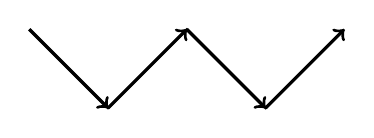
\begin{tikzpicture}
        % define point
        \coordinate (A)  at (1, 1);
        \coordinate (O)  at (2, 0);
        \coordinate (B)  at (3, 1);
        \coordinate (C)  at  (4,0);
        \coordinate (D) at  (5,1);
        % angle  
        \draw[thick] (A) -- (O) -- (B) -- (C)-- (D);
        \draw [->, very thick] (1,1) -- (2,0)  node [midway, above] {\scriptsize };
        \draw [->, very thick] (2,0) -- (3,1)  node [midway, above] {\scriptsize };
        \draw [->, very thick] (3,1) -- (4,0)  node [midway, above] {\scriptsize };
        \draw [->, very thick] (4,0) -- (5,1)  node [midway, above] {\scriptsize };
    \end{tikzpicture}
    \captionof{figure}{Gesture Wing}
\end{center}


The letter \textbf{W} is composed by 4 little movement : 

\begin{itemize}
    \item The device is first moved down and to the right.
    \item Then the device is moved up and to the right.
    \item The device is then moved down and to the right.
    \item  The device is then moved up and to the right again. 
\end{itemize}


\subsection{Gesture Ring}

The gesture Ring is composed by circular motion.  

\begin{center}
    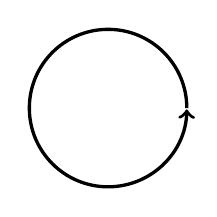
\begin{tikzpicture}
        \draw[->,very thick] (0,0) arc[radius=1cm,start angle=0,delta angle=359];
    \end{tikzpicture}
    
    \captionof{figure}{Gesture Ring}	
\end{center}
The process involved in capturing gesture Ring are as follows.
\begin{itemize}
    \item Trace a clockwise circle using the wand.
    \item Aim again to take around a second to perform gesture.	
    \item The gesture Ring is a rotation of wirst and not shoulder.
\end{itemize}


\subsection{Gesture Slope}

\begin{center}	
    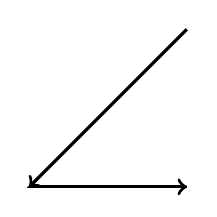
\begin{tikzpicture}	
        \coordinate (A)  at (2, 2);
        \coordinate (O)  at (0, 0);
        \coordinate (B)  at (2, 0);
        
        \draw[thick] (A) -- (O) -- (B);
        \draw [->, very thick] (2,2) -- (0,0)  node [midway, above] {\scriptsize };
        \draw [->, very thick] (0,0) -- (2,0)  node [midway, above] {\scriptsize };
    \end{tikzpicture}
    
    \captionof{figure}{Gesture Slope}
    
\end{center}
The steps involved in waving the gesture Slope  is mentioned below.
\begin{itemize}
    
    \item The device is first moved down and to the left.
    \item Then the device is moved to the right.
    \item Finally you should get a corner of the triangle as shown in the figure.
    
\end{itemize}

The movement recognized is possible after train each part, each movement. If we do Slope on left or on right it's different movement.

Some problem can appart when you try to do the movement, the problem  is the gesture Slope is always detect. 

The movements based on Wrist and shoulder are different, although they can give similar results, so it's essential to focus on training. Depending on the training, one of the two will stand out. 


\section{Magic Wand gear}

The magic wand is composed by different things : 

\begin{itemize}
    \item the Arduino Nano 33 BLE Sense card:
    
    \URL{https://docs.arduino.cc/hardware/nano-33-ble/}
    
    \item The Acrylic stick: 
    
    \URL{https://data.energizer.com/pdfs/cr2032.pdf}
    
    \item The button pile CR2032 on Lithium:
    
    \URL{https://data.energizer.com/pdfs/cr2032.pdf}
    
    \item PETG filament was used for 3D printing: 
    
    \URL{https://www.material4print.de/filament/petg/31/petg-tiefschwarz?c=15} 
    
\end{itemize}

After the choice of this different things we need to devellop how it's used. 

\subsection{Arduino Nano 33 BLE Sense}

The Arduino board remains unchanged, with links to the battery and jumper to be detailed later. 

The Arduino project is unchanged in most cases. The only change is in the file \FILE{arduino\_output\_handler.cpp}.

\begin{center}
    \captionof{code}{Arduino Modification}
    \ArduinoExternal{firstline=16, lastline=30}{../../Code/Nano33BLESense/magic_wand_code/arduino_output_handler.cpp}
    \label{Code:ArduinoModif}
\end{center}

This part have some modification about the creation of timer, it had a \PYTHON{CycleTimeOn} and \PYTHON{CycleTimeOff}, and other feature. 

\begin{center}
    \captionof{code}{Arduino Modification 2}
    \ArduinoExternal{firstline=33, lastline=64}{../../Code/Nano33BLESense/magic_wand_code/arduino_output_handler.cpp}
    \label{Code:ArduinoModif2}
\end{center}

This part of code containt the switch of color for 0.5 second OFF and 0.5 second ON. It serial.println some value to understand the changement of value. The color change 3 times, it s go on red to green to blue. 

\begin{center}
    \captionof{code}{Arduino Modification 3}
    \ArduinoExternal{firstline=68, lastline=75}{../../Code/Nano33BLESense/magic_wand_code/arduino_output_handler.cpp}
    \label{Code:ArduinoModif3}
\end{center}


During the initilisation the pin of led color on Red, Green and Blue is define on OUTPUT. 


\begin{center}
    \captionof{code}{Arduino Modification 4}
    \ArduinoExternal{firstline=78, lastline=106}{../../Code/Nano33BLESense/magic_wand_code/arduino_output_handler.cpp}
    \label{Code:ArduinoModif4}
\end{center}

This part of code show the color when the movement change when it's gesture Wing it's red color, when it's gesture Ring it's green color and for gesture Slope it's blue. 

If no movement is recognize, the last part of the code run and the color past on red to green to blue and cut. They past 0.5 second \textcolor{violet}{OFF} and 0.5 second \textcolor{violet}{ON}. 

\begin{center}
    \captionof{code}{Arduino Modification 5}
    \ArduinoExternal{firstline=107, lastline=115}{../../Code/Nano33BLESense/magic_wand_code/arduino_output_handler.cpp}
    \label{Code:ArduinoModif5}
\end{center}


After seeing the program we saw modification about the code to adapt in your program. Now we need to create the support of magic wand. 

\subsection{Magic Wand support}

The magic wand is composed of 2 major part : 

\begin{itemize}
    \item Acrylic stick
    \item Card and stick support
\end{itemize}

The acrylic stick can be found on internet, with the link behind. The card and stick support was created on PETG filament with 3D printing. During the 3D printing, the direction of printing will influence the ability to absorb shock in traction or shear. 


For our project, 3D printing shouldn't be important, although a horizontal print will better withstand the stresses exerted by the stick during movement. The support of magic wand is composed by 3 part, the high part, the low part and mid part. 


The high part is define on schema \ref{Figure:Fusion360Schema1} and a drawing \ref{Figure:Fusion360Draw1} as defined \cite{Fusion:2024} below: 

\begin{center}
    \includegraphics[width=8cm]{MagicWand/fusionHautS.png}
    \captionof{figure}{Support schema of high part} \label{Figure:Fusion360Schema1}	
\end{center}

\begin{center}
    \includegraphics[width=8cm]{MagicWand/fusionHautD.png}
    \captionof{figure}{Support drawing of high part} \label{Figure:Fusion360Draw1}	
\end{center}


The low part is define on schema \ref{Figure:Fusion360Schema2} and a drawing \ref{Figure:Fusion360Draw2} as defined \cite{Fusion:2024b} below: 

\begin{center}
    \includegraphics[width=8cm]{MagicWand/fusionBasS.png}
    \captionof{figure}{Support schema of low part} \label{Figure:Fusion360Schema2}	
\end{center}

\begin{center}
    \includegraphics[width=8cm]{MagicWand/fusionBasD.png}
    \captionof{figure}{Support drawing of low part} \label{Figure:Fusion360Draw2}	
\end{center}

The mid part is define on different schema \ref{Figure:Fusion360Schema3} \ref{Figure:Fusion360Schema4} and a drawing \ref{Figure:Fusion360Draw3} \ref{Figure:Fusion360Draw4}. On this schema we need to payed intention for the cut to the arduino card. This part is defined with the schema \cite{Fusion:2024c} below: 

\begin{center}
    \includegraphics[width=7cm]{MagicWand/fusionMidS2.png}
    \captionof{figure}{Support schema of low part} \label{Figure:Fusion360Schema3}	
\end{center}

\begin{center}
    \includegraphics[width=6cm]{MagicWand/fusionMidD1.png}
    \captionof{figure}{Support drawing of low part} \label{Figure:Fusion360Draw3}	
\end{center}

\begin{center}
    \includegraphics[width=5.5cm]{MagicWand/fusionMidS1.png}
    \captionof{figure}{Support schema of low part} \label{Figure:Fusion360Schema4}	
\end{center}

\begin{center}
    \includegraphics[width=5.5cm]{MagicWand/fusionMidD2.png}
    \captionof{figure}{Support drawing of low part} \label{Figure:Fusion360Draw4}	
\end{center}

The mid extarnal part is define on schema \ref{Figure:Fusion360Schema5} and a drawing \ref{Figure:Fusion360Draw5} as defined \cite{Fusion:2024d} below: 

\begin{center}
    \includegraphics[width=7cm]{MagicWand/fusionMidExtS.png}
    \captionof{figure}{Support schema of mid external part} \label{Figure:Fusion360Schema5}	
\end{center}

\begin{center}
    \includegraphics[width=5cm]{MagicWand/fusionMidExtD.png}
    \captionof{figure}{Support drawing of mid external part} \label{Figure:Fusion360Draw5}	
\end{center}

\subsection{3D printing}

The 3D printing is a part of the project. The additive manufacturing using fused deposition modeling is the correct name of our impression, but in current time we said "3D printing". It will be realized by PrusaSlicer, a 3D printing software. 

It's a complex process, which is carried out layer by layer, so it's important to note that some support is required for the project to run smoothly. Some parts don't directly touch the printer deck or its opening, so we need to create an organic support to hold the structure in place. The program sent to the machine is in G-code. 

\begin{center}
    \includegraphics[width=6cm]{MagicWand/STLfile}
    \captionof{figure}{STL file}
\end{center}

First of all, you need to create a file in STL format,when you do this file you need to add some requirement like the refining, a high level of refining can give a circle like a circle and a low level it must be a hexagonal form, you can do some specific modification if you don't like the automatique mode.

\begin{center}
    \includegraphics[width=9cm]{MagicWand/PrusaPrint}
    \captionof{figure}{Prusa Slicer example print}
\end{center}

After do this, we can import the file to PrusaSlicer, then we can slash the file, to do a simulation and after this you check if we don't have problem. The major problem can be arrived with the support size. If all is good, we can export the G-code to the printer hub. If we have some problem we juste need to modify the position of the code. 


It's also important to note that extrusion speed and the temperature at which the wire or deck is heated will have an impact on print quality. 

For our impression, we used a based at 60°C and file at 225°C, for the speed it's not so  speed, about at 40 mm/s. 

3D printing can take several hours, so don't hesitate to check your results before printing. 

\begin{center}
    \includegraphics[width=6cm]{MagicWand/PrusaSlicer}
    \captionof{figure}{Prusa Slicer example print}
\end{center}


\subsection{Magic Wand Battery}

The battery off Magic Wand is a button battery CR2032 on Lithium, to used correctly the batterie we need a specifique connection. This battery connection is also connect on Power button. 

The battery need some description about the capacity, the current voltage for Arduino Nano 33 BLE Sense battery is about 3.3V. The button cell batteries can have a capacity of up to 3.7V, making them ideal for the Arduino Nano, since they are only used occasionally. The voltage will then vary between 3V when it's full and 2.6V when it's empty. 


The connection betwin battery and card is something particular with the power button, we connect the battery and the card like this :  

\begin{itemize}
    \item The positive part of the battery is connected to one part of the ON/OFF button.
    \item The second part of the ON/OFF button is connected to the +3.3V battery. 
    \item The negative go to arduino gnd to button battery gnd. 
\end{itemize}


\subsection{Magic Wand Jumper}

The jumper consists of two wires that never touch. When the jumper is not activated, either the two wires are touching, or there is no soldering and the jumper is not cut; this case is effective when there is no battery. 
When a battery is added, the jumper is set \ref{Figure:JumperPhoto}, preventing the creation of a short circuit.

The battery's GND is on the board's GND (in black) and the battery's 3V is on the board's 3.3V. The jumper, on the other hand, is “in a vacuum”, and the battery and jumper connections are defined by the board below \ref{Figure:jumperconnection}. 

The creation and installation of this jumper is essential to the operation of the battery. Without the jumper in place, the arduino board would be in danger. 
\begin{center}
    \includegraphics[width=4cm]{MagicWand/jumper}
    \captionof{figure}{Jumper connection Arduino card}
    \label{Figure:jumperconnection}
    
    \bigskip
    
    \includegraphics[width=5cm]{MagicWand/jumperphoto}
    \captionof{figure}{Photo of the jumper on the project}
    \label{Figure:JumperPhoto}
\end{center} 